\chapter{Introduction}
\label{chp:introduction} 

This section is intended to provide an overview of the contents and context of this report. The first part of this section gives a brief introduction to the field of mobile autonomous robotics and computer vision, as well as the benifits and potential applications for this technology. The robot system and tools used in the project is presented in subsection \ref{}. Lastly, each of the following sections will given short introductions.




\section{Mobile Autonomous Robotics and Computer Vision}

Put the task into a larger context. Bring in some points on the societal impact of autonomous robotics and the increased potential of mobile robotics.  

The field of computer vision has seen an enormous growth over the last few decades - not only in scale, but in accessibility and capability as well. As a consequence of this recent growth, tapping into the field of computer vision is bound to reveal applications that are useful for a mobile autonomous maintenance robot. Recent discoveries within computer vision includes robust feature recognition and object detection, face detection and video processing. The latest great additions to the field are Big Data and Artificial Intelligence.

\section{System Overview}

The mobile robot being worked on in this project is shown in figure \ref{fig:RobotFront}. The manipulator arm  has been used in previous projects on robotic maintenance, and it was placed on the mobile platform during the master thesis of (Aspunvik og siter). This section provides a short description of the hardware. If a more detailed description of the robot and it's equipment is required, consult the thesis of Aspunvik[cite]. 

\begin{figure}
\centering
 \begin{subfigure}[b]{0.3\textwidth}
        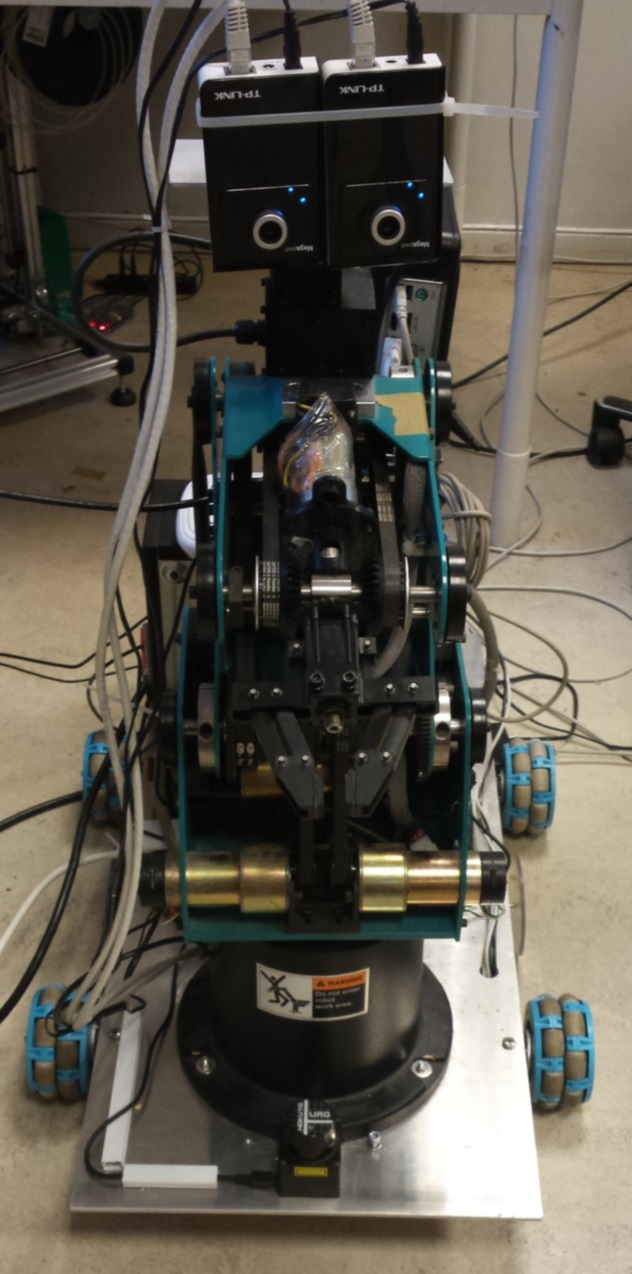
\includegraphics[width=\textwidth]{Robot_front}
        \caption{Front view.}
        \label{fig:RobotFront}
    \end{subfigure}
    \begin{subfigure}[b]{0.65\textwidth}
        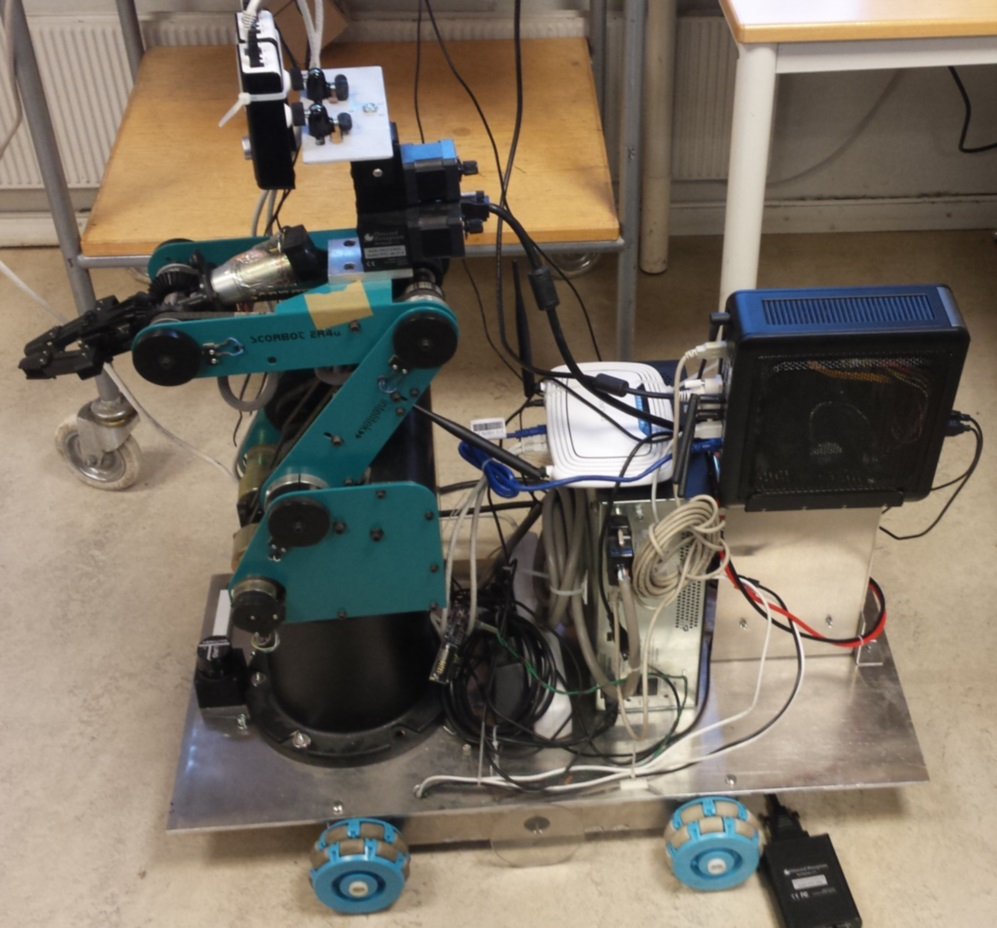
\includegraphics[width=\textwidth]{Robot_side}
        \caption{Side view.}
        \label{fig:RobotSide}
    \end{subfigure}
    \caption{\label{fig:RobotView}The robot used in the project.}
\end{figure}

\subsection{Propulsion}

The steel chassis of the robot stands upon four omni-wheels. The wheel pairs are placed in parallel, making the vehicle uncontrollable along the lateral axis. Each wheel is powered by an electrical motor and motor driver. The motor drivers are controlled with pulse width modulation by an evaluation board from Atmel,(atmel kort).  

\subsection{Sensors}

The robot was outfitted with several sensors during previous projects. These are:
\begin{itemize}
	\item Two odometer wheels with encoders. One on each side. 
	\item Two infrared distance sensors. 
	\item A LIDAR (Light Detection and Ranging).
	\item Two IP-cameras.
\end{itemize} 

Only the cameras were used in this projects. 

\subsection{The Manipulator}



\begin{figure}
	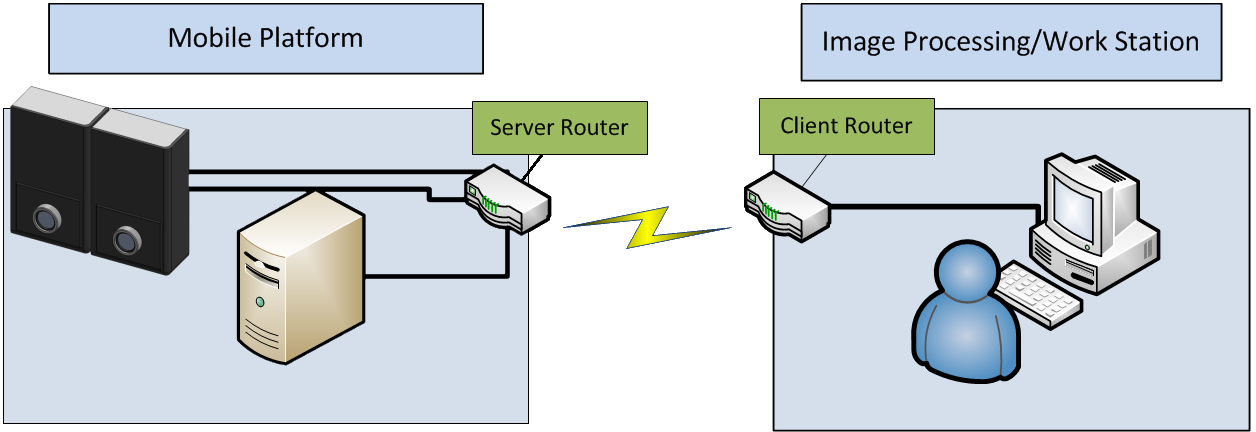
\includegraphics[width=1\textwidth]{hardwareSetup_cropped}
\end{figure}

\section{Report Structure}
How the report is structured, and a very brief description of the contents in each section.